%%%%%%%%%%%%%%%%%%%%%%%%%%%%%%%%%%%%%%%%%%%%%%%%%%%%%%%%%%%%%%%%%%%
%%%%%%%%%%%%%%%%%%%%%%%%%%%%%%%%%%%%%%%%%%%%%%%%%%%%%%%%%%%%%%%%%%%
\begin{frame}{Alternatives to overcome quadrature problems}


\begin{thebibliography}{1}
\bibitem{JAnder}Rivera, J.A., Taylor, J.M., Omella, Á.J., Pardo, D.: On quadrature rules for solving Partial Differential Equations using Neural Networks, Computer Methods in Applied Mechanics and Engineering, \textbf{393}, 114710 (2022).
\end{thebibliography}

\vspace{0.7cm}

\begin{itemize}
\item Monte Carlo integration (and its variants)
\vspace{0.2cm}
\item Explainability of the NN: Regularisation methods
\vspace{0.2cm}
\item $h$-adaptive integration
\vspace{0.2cm}
\item Piecewise-polynomial approximation
\end{itemize}


\end{frame}
%%%%%%%%%%%%%%%%%%%%%%%%%%%%%%%%%%%%%%%%%%%%%%%%%%%%%%%%%%%%%%%%%%%
%%%%%%%%%%%%%%%%%%%%%%%%%%%%%%%%%%%%%%%%%%%%%%%%%%%%%%%%%%%%%%%%%%%
%%%%%%%%%%%%%%%%%%%%%%%%%%%%%%%%%%%%%%%%%%%%%%%%%%%%%%%%%%%%%%%%%%%
\begin{frame}{Monte Carlo integration}
\begin{center}
$
\ds \int_a^b f(x) dx \approx \frac{b-a}{N} \sum_{i=1}^N f(X_i), \;
$
where $X \sim Uniform(a,b)$
\end{center}

\begin{columns}
\begin{column}{0.8\textwidth}
\begin{itemize}
\item[\tickYes] Convergence rate independent of the dimension: $\mathcal{O}(N^{-1/2})$
\item[\tickNo] Slow convergence in low dimensions (1D, 2D, 3D)
\item[\tickYes] Appropriate for high dimensions
\item[\tickYes] Mesh-free method
\item[\tickYes] Allows the use of autodiff to compute $\nabla u$
\item[\tickYes] Easy to implement
\item[\tickYes] Exploit the use of minibatches and GPUs
\end{itemize}
\end{column}
%
\begin{column}{0.2\textwidth}
\vspace{-2.2cm}
\hspace{-3cm}
\includegraphics[scale=1.2]{frames/Javi/img/casino.jpg}

    \end{column}
\end{columns}
\end{frame}
%%%%%%%%%%%%%%%%%%%%%%%%%%%%%%%%%%%%%%%%%%%%%%%%%%%%%%%%%%%%%%%%%%%%
%%%%%%%%%%%%%%%%%%%%%%%%%%%%%%%%%%%%%%%%%%%%%%%%%%%%%%%%%%%%%%%%%%%

%\begin{frame}{Explainability of the NN: Regularisation methods}
%
%\only<1-1>{
%
%\centering
%
%\begin{itemize}
%\vspace{0.2cm}
%\item The midpoint rule has an error estimate 
%
%$$\left|\int_{a}^b \eta(x)\,dx - \sum\limits_{i=1}^N \frac{b-a}{N}\eta(x_i)\right|\leq \frac{(b-a)^2}{2N^2}\sum\limits_{i=1}^N\max\limits_{x\in K_i}|\eta'(x_i)|.$$
%
%\vspace{0.2cm}
%
%\item We can control the quadrature error by controlling $\frac{(b-a)^2}{2N^2}\sum\limits_{i=1}^N\max\limits_{x\in K_i}|\eta'(x_i)|$
%\vspace{0.2cm}
%\item We aim to find a function $\mathcal{R}$ so that for $\eta(x)=\frac{1}{2}u'(x)^2-f(x)u(x)$,
%
%\begin{equation*}
%\frac{(b-a)^2}{2N^2}\sum_{i=1}^N\max_{x\in K_i}|\eta'(x_i)|<\mathcal{R}.
%\end{equation*}
%
%\end{itemize}
%}
% 
%\only<2-2>{
%
%\begin{itemize}
%\item Using arguments similar to (Mishra \textit{et al.}, 2020), for a simple NN:
%
%\begin{equation*}
%\mathcal{R}\left(\theta, u_{NN}(x_i), \dfrac{\partial^{n}u_{NN}(x_i) }{\partial x^{n}} \right).
%\end{equation*}
%
%\vspace{0.2cm}
%\item We  minimise the loss:
%\begin{equation*}
%\mathcal{L} = F_{(\cdot)}(u)+\mathcal{R}\left(\theta, u_{NN}(x_i), \dfrac{\partial^{n}u_{NN}(x_i) }{\partial x^{n}} \right).
%\end{equation*}
%
%\vspace{0.2cm}
%\item $\mathcal{R}$ acts as a regulariser, penalising poor quadrature via the loss. 
%\vspace{0.2cm}
%\item $\mathcal{R}\sim \frac{1}{N}$, so for $N$ large, the ``bias" from $\mathcal{R}$ vanishes.
%%
%
%\vspace{0.5cm}
%
%%\beamertemplatebookbibitems
%\begin{thebibliography}{1}
%%\bibitem{Author1990}A. Author. \newblock\emph{Handbook of Everything}.\newblock
%%Some Press, 1990.\beamertemplatearticlebibitems
%\bibitem{Mishra}Mishra, S., Molinaro, R.: Estimates on the generalization error of physics informed neural
%networks (PINNs) for approximating PDEs. ArXiv:2006.16144 (2020).
%\end{thebibliography}
%
%\end{itemize}
%}
%
%\end{frame}
%%%%%%%%%%%%%%%%%%%%%%%%%%%%%%%%%%%%%%%%%%%%%%%%%%%%%%%%%%%%%%%%%%%%
\begin{frame}{Explainability of the NN: Regularisation methods}
\centering

\begin{itemize}
\item We  minimise the loss:
$$\mathcal{L}_{total} = \mathcal{L}_{Ritz}+\mathcal{R}.$$
\vspace{0.2cm}

\item Using arguments similar to (Mishra \textit{et al.}, 2020), we define $\mathcal{R}$ for a simple NN as:

\begin{equation*}
\mathcal{R}\left(\theta, u_{NN}(x_i), \dfrac{\partial^{n}u_{NN}(x_i) }{\partial x^{n}} \right).
\end{equation*}


\vspace{0.2cm}
\item $\mathcal{R}$ acts as a regulariser, penalising poor quadrature via the loss. 
%\vspace{0.2cm}
%\item $\mathcal{R}\sim \frac{1}{N}$, so for $N$ large, the ``bias" from $\mathcal{R}$ vanishes.
%

\vspace{0.5cm}

%\beamertemplatebookbibitems
\begin{thebibliography}{1}
%\bibitem{Author1990}A. Author. \newblock\emph{Handbook of Everything}.\newblock
%Some Press, 1990.\beamertemplatearticlebibitems
\bibitem{Mishra}Mishra, S., Molinaro, R.: Estimates on the generalization error of physics informed neural
networks (PINNs) for approximating PDEs. ArXiv:2006.16144 (2020).
\end{thebibliography}

\end{itemize}

\end{frame}
%%%%%%%%%%%%%%%%%%%%%%%%%%%%%%%%%%%%%%%%%%%%%%%%%%%%%%%%%%%%%%%%%%%%
%\begin{frame}{Explainability of the NN: Regularisation methods \textcolor{red}{compressed 2in1}}
%\centering
%
%\begin{itemize}
%
%\item The midpoint rule has an error estimate 
%$$\left|\int_{a}^b \eta(x)\,dx - \sum\limits_{i=1}^N \frac{b-a}{N}\eta(x_i)\right|
%\leq 
%\overbrace{\frac{(b-a)^2}{2N^2}\sum\limits_{i=1}^N\max\limits_{x\in K_i}|\eta'(x_i)|}^{\textcolor{blue}{Q}}.$$
%
%\vspace{0.2cm}
%
%\item We find a function $\mathcal{R}$ to control de error for $\eta(x)=\frac{1}{2}u'(x)^2-f(x)u(x)$,
%$$\textcolor{blue}{Q} < \mathcal{R}\left(\theta, u_{NN}(x_i), \dfrac{\partial^{n}u_{NN}(x_i) }{\partial x^{n}} \right).  $$
%
%\vspace{0.2cm}
%
%\item $\mathcal{R}$ acts as a regulariser, penalising poor quadrature via the loss:
%
%$$\mathcal{L}_{total} = \mathcal{L}_{Ritz}+\mathcal{R}.$$
%\end{itemize}
%
%\end{frame}
%%%%%%%%%%%%%%%%%%%%%%%%%%%%%%%%%%%%%%%%%%%%%%%%%%%%%%%%%%%%%%%%%%%%
\begin{frame}{Explainability of the NN: Regularisation methods}
\vspace{0.25cm}
\begin{itemize}
\item[\tickYes]The loss prohibits overfitting
\vspace{0.15cm}

\item[\tickYes] We have {\it a posteriori} estimation of quadrature error
\vspace{0.15cm}

\item[\tickYes] $\mathcal{R}$ is computationally cheap to evaluate
\vspace{0.15cm}
%
\item[\tickNo] If $N$ is small, the problem is drastically changed by $\mathcal{R}$
\vspace{0.15cm}

\item[\tickNo] Finding an expression for $\mathcal{R}$ is difficult and problem dependent
\vspace{0.15cm}

\item[\tickNo] Only valid for regular integrands
\end{itemize}

\end{frame}
%%%%%%%%%%%%%%%%%%%%%%%%%%%%%%%%%%%%%%%%%%%%%%%%%%%%%%%%%%%%%%%%%%%
%%%%%%%%%%%%%%%%%%%%%%%%%%%%%%%%%%%%%%%%%%%%%%%%%%%%%%%%%%%%%%%%%%%
%%%%%%%%%%%%%%%%%%%%%%%%%%%%%%%%%%%%%%%%%%%%%%%%%%%%%%%%%%%%%%%%%%%
%%%%%%%%%%%%%%%%%%%%%%%%%%%%%%%%%%%%%%%%%%%%%%%%%%%%%%%%%%%%%%%%%%%
\begin{frame}{$h$-adaptive integration}
\centering
\begin{tikzpicture}
\only<1->{
\node at (0,1) {};
\node at (12,-6) {};
% TRAIN
\draw (0,0) -- (8,0);

\draw[red,fill=red] (0,0) circle (0.7ex);
\draw[violet,fill=violet] (8,0) circle (0.7ex);
\node [red] at (0,-0.4){$\Gamma_D$};
\node [violet] at (8,-0.4){$\Gamma_N$};

\foreach \Point in {(2,0), (4,0), (6,0)}{\draw[fill=black] \Point circle (0.5ex);}
%\node at (0,-0.25) {$a$};
%\node at (8,-0.25) {$b$};
%%
%%
% VALIDATION
\draw (0,-3) -- (8,-3);

\draw[red,fill=red] (0,-3) circle (0.7ex);
\draw[violet,fill=violet] (8,-3) circle (0.7ex);
\node [red] at (0,-3.4){$\Gamma_D$};
\node [violet] at (8,-3.4){$\Gamma_N$};

\foreach \Point in {((2,-3), (4,-3), (6,-3),(1,-3), (3,-3), (5,-3), (7,-3)}{\draw[fill=black] \Point circle (0.5ex);}
%\foreach \Point in {(0,-3), (2,-3), (4,-3), (6,-3), (8,-3)}{\node at \Point {\textbullet};}
%\foreach \Point in {(1,-3), (3,-3), (5,-3), (7,-3)}{\node[violet] at \Point {\textbullet};}
%\node at (0,-3.25) {$a$};
%\node at (8,-3.25) {$b$};

\node at (11,0) {Training};
\node at (11,-3) {Validation};
};

\only<1>{
\shade[shading=ball, ball color=structure] (-0.1,-4.95) circle (.1);
\node [anchor = west]at (0,-5) {We define two meshes};
};

%
\only<1-2>{
% TRAIN
\draw[<->, dashed] (0,0.5) -- (2,0.5);
\node at (1,0.75) {$h$};
% VALIDATION
\draw[<->, dashed] (0,-2.5) -- (1,-2.5);
\node at (0.5,-2.25) {$h/2$};
};

\only<2>{
% TRAIN
\node [draw, circle, blue ,  inner sep=-1.2] (G1K1) at (0.2254, 0){};
\node [draw, circle, blue ,  inner sep=-1.2] (G2K1) at (1, 0)   {};
\node [draw, circle, blue ,  inner sep=-1.2] (G3K1) at (1.7746, 0){};

\node [draw, circle, blue ,  inner sep=-1.2] (G1K2) at (2+0.2254, 0){};
\node [draw, circle, blue ,  inner sep=-1.2] (G2K2) at (2+1, 0)   {};
\node [draw, circle, blue ,  inner sep=-1.2] (G3K2) at (2+1.7746, 0){};

\node [draw, circle, blue ,  inner sep=-1.2] (G1K3) at (4+0.2254, 0){};
\node [draw, circle, blue ,  inner sep=-1.2] (G2K3) at (4+1, 0)   {};
\node [draw, circle, blue ,  inner sep=-1.2] (G3K3) at (4+1.7746, 0){};

\node [draw, circle, blue ,  inner sep=-1.2] (G1K4) at (6+0.2254, 0){};
\node [draw, circle, blue ,  inner sep=-1.2] (G2K4) at (6+1, 0)   {};
\node [draw, circle, blue ,  inner sep=-1.2] (G3K4) at (6+1.7746, 0){};
%
%% VALIDATION
\node [draw, circle, blue ,  inner sep=-1.2] (VG1K1) at (0.2254/2, -3){};
\node [draw, circle, blue ,  inner sep=-1.2] (VG2K1) at (1/2, -3)   {};
\node [draw, circle, blue ,  inner sep=-1.2] (VG3K1) at (1.7746/2, -3){};
%
\node [draw, circle, blue ,  inner sep=-1.2] (VG1K1b) at (1+0.2254/2, -3){};
\node [draw, circle, blue ,  inner sep=-1.2] (VG2K1b) at (1+1/2, -3)   {};
\node [draw, circle, blue ,  inner sep=-1.2] (VG3K1b) at (1+1.7746/2, -3){};

\node [draw, circle, blue ,  inner sep=-1.2] (VG1K2) at (2+0.2254/2, -3){};
\node [draw, circle, blue ,  inner sep=-1.2] (VG2K2) at (2+1/2, -3)   {};
\node [draw, circle, blue ,  inner sep=-1.2] (VG3K2) at (2+1.7746/2, -3){};
%
\node [draw, circle, blue ,  inner sep=-1.2] (VG1K2b) at (3+0.2254/2, -3){};
\node [draw, circle, blue ,  inner sep=-1.2] (VG2K2b) at (3+1/2, -3)   {};
\node [draw, circle, blue ,  inner sep=-1.2] (VG3K2b) at (3+1.7746/2, -3){};

\node [draw, circle, blue ,  inner sep=-1.2] (VG1K3) at (4+0.2254/2, -3){};
\node [draw, circle, blue ,  inner sep=-1.2] (VG2K3) at (4+1/2, -3)   {};
\node [draw, circle, blue ,  inner sep=-1.2] (VG3K3) at (4+1.7746/2, -3){};
%
\node [draw, circle, blue ,  inner sep=-1.2] (VG1K3b) at (5+0.2254/2, -3){};
\node [draw, circle, blue ,  inner sep=-1.2] (VG2K3b) at (5+1/2, -3)   {};
\node [draw, circle, blue ,  inner sep=-1.2] (VG3K3b) at (5+1.7746/2, -3){};

\node [draw, circle, blue ,  inner sep=-1.2] (VG1K4) at (6+0.2254/2, -3){};
\node [draw, circle, blue ,  inner sep=-1.2] (VG2K4) at (6+1/2, -3)   {};
\node [draw, circle, blue ,  inner sep=-1.2] (VG3K4) at (6+1.7746/2, -3){};
%
\node [draw, circle, blue ,  inner sep=-1.2] (VG1K4b) at (7+0.2254/2, -3){};
\node [draw, circle, blue ,  inner sep=-1.2] (VG2K4b) at (7+1/2, -3)   {};
\node [draw, circle, blue ,  inner sep=-1.2] (VG3K4b) at (7+1.7746/2, -3){};

%\node [blue](G) at (4,-1.5){Gauss points};
%
%\draw[->, blue] (G) edge (G2K1);
%\draw[->, blue] (G) edge (G2K2);
%\draw[->, blue] (G) edge (G3K2);
%\draw[->, blue] (G) edge (G2K4);
%
%\draw[->, blue] (G) edge (VG2K1);
%\draw[->, blue] (G) edge (VG2K2);
%\draw[->, blue] (G) edge (VG3K2b);
%\draw[->, blue] (G) edge (VG2K4);

\shade[shading=ball, ball color=structure] (-0.1,-4.95) circle (.1);
\node [anchor = west]at (0,-5) {We select a three-point Gaussian quadrature};

};
%
\only<3>{
\draw [orange, decorate, decoration = {brace,mirror}] (0,-0.5) -- (2,-0.5)node[pos=0.5,below=3pt,black]{$I_{1}$};

\draw [violet, decorate, decoration = {brace,mirror}] (2,-0.5) -- (4,-0.5)node[pos=0.5,below=3pt,black]{$I_{2}$};

\draw [green!30!black, decorate, decoration = {brace,mirror}] (4,-0.5) -- (6,-0.5)node[pos=0.5,below=3pt,black]{$I_{3}$};

\draw [brown, decorate, decoration = {brace,mirror}] (6,-0.5) -- (8,-0.5)node[pos=0.5,below=3pt,black]{$I_{4}$};
%
\draw [orange, decorate, decoration = {brace}] (0,-2.75) -- (1,-2.75)node[pos=0.5,above=3pt,black]{$I_{1,1}$};
\draw [orange, decorate, decoration = {brace}] (1,-2.75) -- (2,-2.75)node[pos=0.5,above=3pt,black]{$I_{1,2}$};
\node at (1, -2.25) {$+$};
\node at (1, -1.55) {\textcolor{red}{$\not\approx$}};

\draw [violet, decorate, decoration = {brace}] (2,-2.75) -- (3,-2.75)node[pos=0.5,above=3pt,black]{$I_{2,1}$};
\draw [violet, decorate, decoration = {brace}] (3,-2.75) -- (4,-2.75)node[pos=0.5,above=3pt,black]{$I_{2,2}$};
\node at (3, -2.25) {$+$};
\node at (3, -1.55) {\textcolor{green!20!black}{$\approx$}};

\draw [green!30!black, decorate, decoration = {brace}] (4,-2.75) -- (5,-2.75)node[pos=0.5,above=3pt,black]{$I_{3,1}$};
\draw [green!30!black, decorate, decoration = {brace}] (5,-2.75) -- (6,-2.75)node[pos=0.5,above=3pt,black]{$I_{3,2}$};
\node at (5, -2.25) {$+$};
\node at (5, -1.55) {\textcolor{red}{$\not\approx$}};

\draw [brown, decorate, decoration = {brace}] (6,-2.75) -- (7,-2.75)node[pos=0.5,above=3pt,black]{$I_{4,1}$};
\draw [brown, decorate, decoration = {brace}] (7,-2.75) -- (8,-2.75)node[pos=0.5,above=3pt,black]{$I_{4,2}$};
\node at (7, -2.25) {$+$};
\node at (7, -1.55) {\textcolor{green!20!black}{$\approx$}};

\shade[shading=ball, ball color=structure] (-0.1,-4.45) circle (.1);
\node [anchor = west]at (0,-4.5) {We compute the integration error during training:};
\node [anchor = west]at (0.5,-5.2) {if $|(I_{j,1} +I_{j,2} ) - I_j| > \epsilon \rightarrow$ mark the elements involved};
};

\only<3-4>{
\node at (1, 0.3) {\tickNo};
\node at (5, 0.3) {\tickNo};

\node at (0.5, -3.3) {\tickNo};
\node at (1.5, -3.3) {\tickNo};
\node at (4.5, -3.3) {\tickNo};
\node at (5.5, -3.3) {\tickNo};
};

\only<4>{

%\foreach \Point in {(1,0), (5, 0)}{\node [red] at \Point {\textbullet};}
%\foreach \Point in {(0.5,-3), (1.5,-3), (4.5,-3), (5.5,-3)}{\node[red] at \Point {\textbullet};}
\foreach \Point in {(1,0), (5, 0),(0.5,-3), (1.5,-3), (4.5,-3), (5.5,-3) }{\draw[] \Point circle (0.5ex);}


%
\shade[shading=ball, ball color=structure] (-0.1,-4.95) circle (.1);
\node [anchor = west]at (0,-5) {We refine the elements marked to produce the new meshes};
};
%
\only<5>{
%\foreach \Point in {(1,0), (5, 0)}{\node [black] at \Point {\textbullet};}
%\foreach \Point in {(1,-3), (5, -3)}{\node [black] at \Point {\textbullet};}
%\foreach \Point in {(0.5,-3), (1.5,-3), (4.5,-3), (5.5,-3)}{\node[violet] at \Point {\textbullet};}

\foreach \Point in {(1,0), (5, 0),(0.5,-3), (1.5,-3), (4.5,-3), (5.5,-3) }{\draw[fill=black] \Point circle (0.5ex);}

\shade[shading=ball, ball color=structure] (-0.1,-1.5) circle (.1);
\node [anchor = west]at (0,-1.5) {Continue training until stop criteria};

\node [anchor = west]at (1,-4.3) {\tickNo $\,$ Mesh based};
\node [anchor = west]at (1,-4.8) {\tickYes $\,$ Appropiate for low dimensional problems};
%\node [anchor = west]at (1,-4.8) {\tickYes $\,$ We expect ''''''' convergence};
\node [anchor = west]at (1,-5.3) {\tickYes $\,$ Allows the use of autodiff to compute $\nabla u$ };
\node [anchor = west]at (1,-5.8) {\tickNo $\,$ Amount of data grows after each refinement};
};
\end{tikzpicture}
\end{frame}
%%%%%%%%%%%%%%%%%%%%%%%%%%%%%%%%%%%%%%%%%%%%%%%%%%%%%%%%%%%%%%%%%%%%

%%%%%%%%%%%%%%%%%%%%%%%%%%%%%%%%%%%%%%%%%%%%%%%%%%%%%%%%%%%%%%%%%%%
%%%%%%%%%%%%%%%%%%%%%%%%%%%%%%%%%%%%%%%%%%%%%%%%%%%%%%%%%%%%%%%%%%%
%%%%%%%%%%%%%%%%%%%%%%%%%%%%%%%%%%%%%%%%%%%%%%%%%%%%%%%%%%%%%%%%%%%\\

\begin{frame}{Piecewise-polynomial approximation}

%\begin{itemize}
%\item We define a mesh
%\end{itemize}
%
%\begin{center}
%\begin{tikzpicture}
%\draw (0,0) -- (8,0);
%\draw[red,fill=red] (0,0) circle (0.7ex);
%\draw[violet,fill=violet] (8,0) circle (0.7ex);
%\node [red] at (0,-0.4){$\Gamma_D$};
%\node [violet] at (8,-0.4){$\Gamma_N$};
%%
%\foreach \Point in {(2,0), (4,0), (6,0)}{\draw[fill=black] \Point circle (0.5ex);}
%\end{tikzpicture}
%\end{center}

\begin{itemize}
\item We define a mesh $\mathcal{T}$.
\item We select the degree $p$ of the polynomial.
\item We define the  vector of nodes: $x_{node} (\mathcal{T}, p)$.
\item We build the approximate solution $u_p (x_{node}, u_{NN}(x_{node}))$ .
\end{itemize}

\vspace{0.5cm}
\begin{columns}
%
\begin{column}{0.45\textwidth}
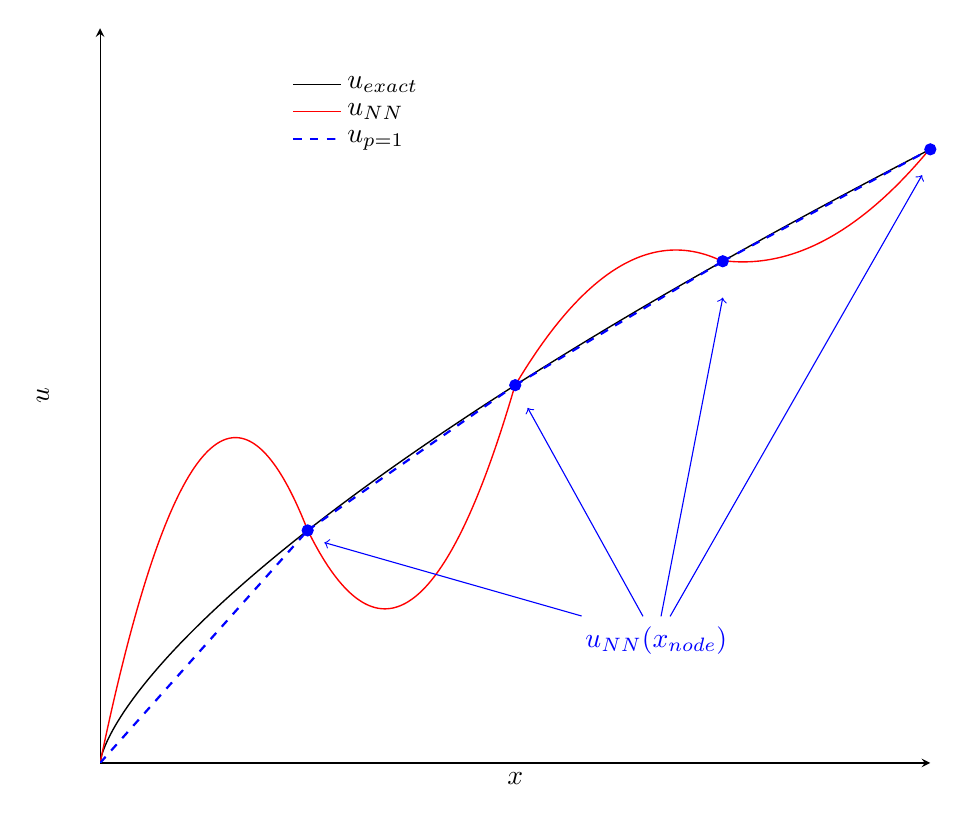
\begin{tikzpicture}
    \begin{axis}[
    xlabel = {$x$},
    xmin=0,
    xmax=10,
    ymin=0,
    ymax=6,
    ylabel = {$u$},
      height=0.9*\textwidth,
      width=1*\textwidth,
    axis lines=left,
    ticks=none,
%    grid=both,
	%xtick={0,0.25,...,1},
	%ytick={0,100},
    %yticklabels={0,$a$},
    y label style={at={(-0.05,0.5)}},
%    xticklabels={-3,-1,...,5},
%    ticks=xticklabels,
    legend columns = 1,
    legend style= {at={(0.4,0.95)},draw=none,fill=none,nodes={scale=1, transform shape}}, legend cell align={left}]
    ]    
    \tikzset{ dot/.style = {circle, fill, minimum size=3pt, inner sep=0pt, outer sep=0pt}, }
% exact 
\addplot[samples=500,color=black, smooth, line width=0.5, domain=0:10] {x^0.7};	
\addlegendentry{$u_{exact}$};

%% u_NN
\addplot[samples=500,color=red, smooth, line width=0.5, domain=0:2.5] {-x^2+3.26*x };
\addlegendentry{$u_{NN}$}
\addplot[samples=10,color=blue, smooth, dashed, domain=0:2.5, line width=0.8] {1.899/2.5*x};
\addlegendentry{$u_{p = 1}$ }
%
%
%%%%%%%% WE NEED TO PUT THE FIRST THREE PLOTS DIFFERENT TO OBTAIN THE CORRECT LEGEND IN THE PLOT
%
%%% u_NN
\addplot[samples=500,color=red, smooth, line width=0.5, domain=2.5:5] {0.743*(x^2)-5.097*x +10};
\addplot[samples=500,color=red, smooth, line width=0.5, domain=5:7.5] {-0.295*(x^2)+4.0918*x -10};
\addplot[samples=500,color=red, smooth, line width=0.5, domain=7.5:10] {0.182*(x^2)-2.818*x +15};

%% u_p
\draw[color=blue, smooth, dashed, line width=0.8] (2.5,1.899) -- (5,3.085);
\draw[color=blue, smooth, dashed, line width=0.8] (5,3.085) -- (7.5,4.097);
\draw[color=blue, smooth, dashed, line width=0.8] (7.5,4.097) -- (10,5.011);

%%points
\addplot[only marks,mark=*,blue,mark size=2pt] coordinates {(2.5,1.899)(5,3.085)(7.5,4.097)(10,5.011)};

    \tikzstyle{state}=[
        draw = white,
        thick,
        fill = white,
        minimum width=15mm, 
        minimum height=4mm
    ]

\node(G)[ state,  ] at (axis cs: 6.7,1.) {\textcolor{blue}{$u_{NN}(x_{node})$}};
%\node(G_aux1)[anchor = north, text width=1.0] at (axis cs: 1.65,31) {};
%\node(G_aux2)[anchor = north, text width=1.0] at (axis cs: 2,31) {};
    

%\node (G1) at (axis cs: 0.28175, 19){};
%\node (G2) at (axis cs: 1.25, 46.27){};
%\node (G3) at (axis cs: 2.21825, 36.05){};
%
%\draw[] (G1) node[above, blue] {};
%\draw[] (G2) node[above, blue] {};
%\draw[] (G3) node[above, blue] {};


\path[->, blue] (axis cs: 5.8,1.2) edge (axis cs:2.7,1.8);
\path[->, blue] (G) edge (axis cs:5.15,2.9);
\path[->, blue] (G) edge (axis cs:7.5,3.8);
\path[->, blue] (G) edge (axis cs:9.9,4.8);

\end{axis}
\end{tikzpicture}
\end{column}
%
\begin{column}{0.55\textwidth}
\begin{itemize}
\item[\tickNo]  Mesh based method
\item[\tickYes] Appropriate for low dimensions
\item[\tickYes] Allows exact integration $\&$ differentiation
\item[\tickNo]  It does not allow the use of autodiff
\item[\tickYes] The amount of data remains constant
\item[\tickYes] Exists theory about its convergence
\end{itemize}
\end{column}
\end{columns}
\end{frame}
%%%%%%%%%%%%%%%%%%%%%%%%%%%%%%%%%%%%%%%%%%%%%%%%%%%%%%%%%%%%%%%%%%%%